%
\section{Workflow}
\label{sec:workflow}
%
\begin{figure}
    \centering
    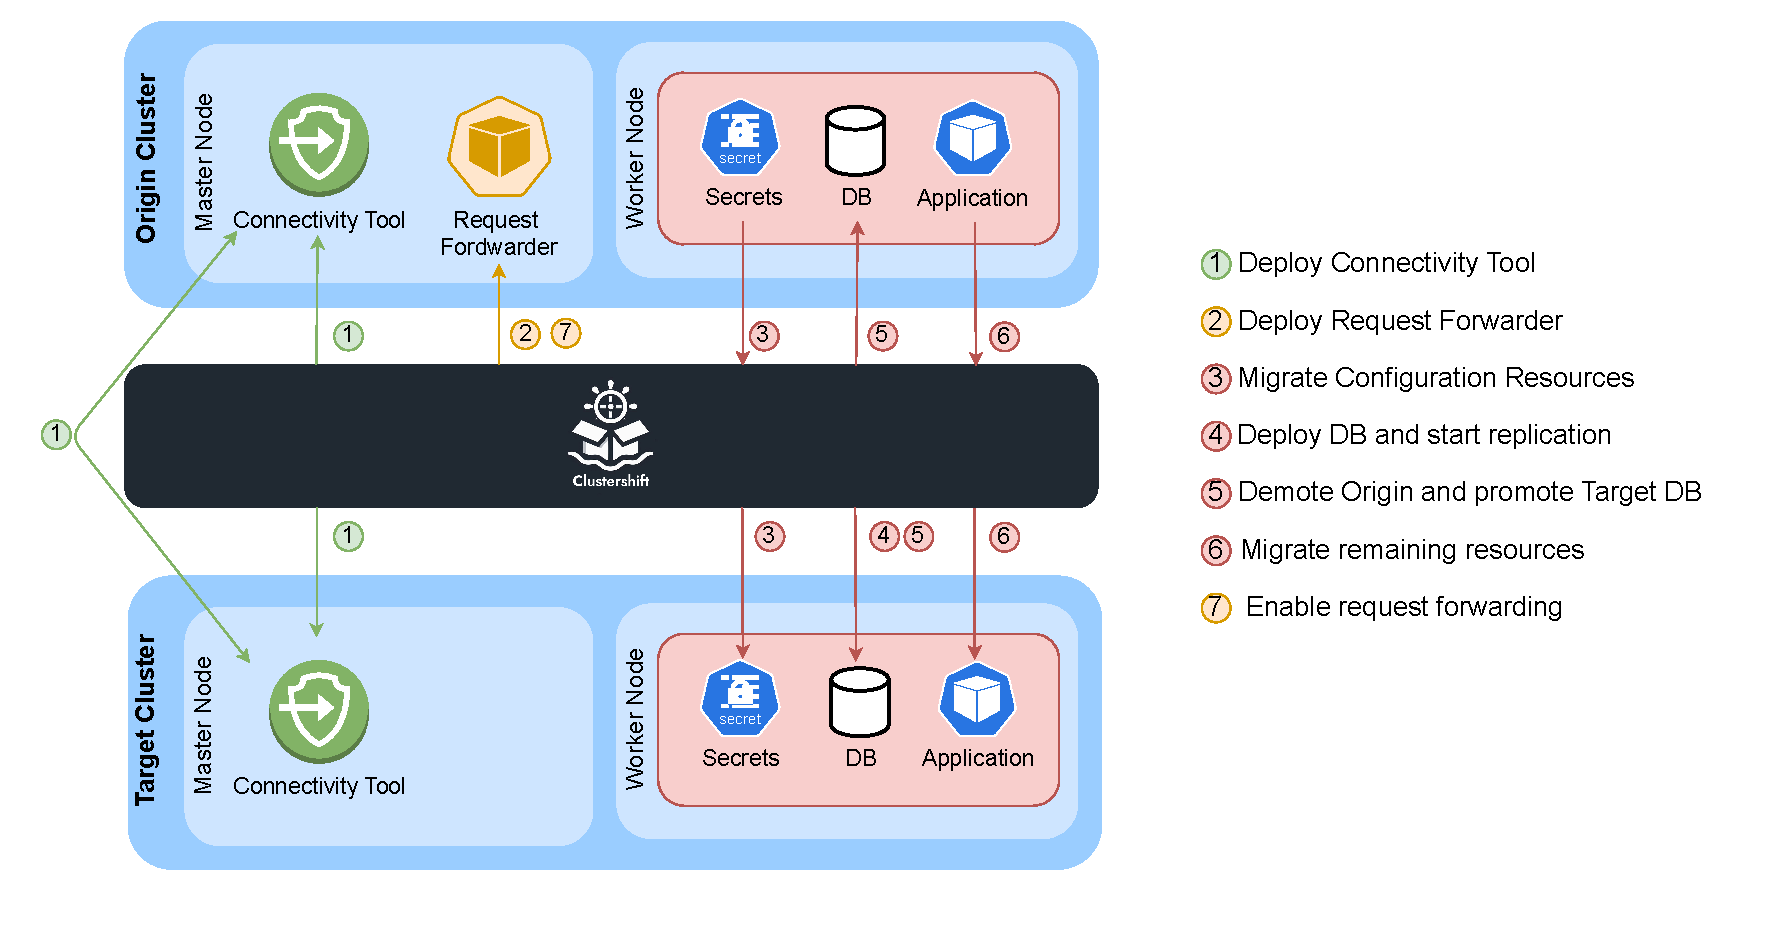
\includegraphics[width=\linewidth]{figures/workflow.pdf}
    \caption{Migration Workflow of Application Stacks with Clustershift.}
    \label{fig:workflow}
\end{figure}
%
In this chapter we take a look at the Workflow of Clustershfit. Figure~\ref{fig:workflow} shows the single steps Clustershift is doing to successfully migrate our application from the origin to the target cluster. Clustershift is running as a command line tool on our local machine accessing both clusters via their kubeconfig.
\paragraph{Step 1} is deploying the connectivity tool. We have the option to deploy submariner, skupper or linkerd. The connectivity tool is there to establish a secure connection between the origin and target cluster. This is getting deployed/installed by Clustershift. After configuring and installing it the connection will be tested via a test application with is getting tried to be accessed from the other cluster. After this is successful the process can continue.
\paragraph{Step 2} is deploying the request forwarder on the origin cluster. It is in an inactive mode and has to be enabled in a different step so the traffic is still being processed by the origin cluster. This is only needed if we are using Custom Reverse Proxy. For our other request forwarding options this step can be ignored. This is also done by Clustershift.
\paragraph{In Step 3} Clustershift is getting all migration configuration resources from the origin cluster. This includes secrets, configmaps, service accounts and other stuff. This is done by using the kubernetes api. These resources are getting cleaned and deployed identically on the target cluster. This step has to be done because the database, application and other resources depend on them.
\paragraph{In Step 4} Clustershift is scanning for running databases on the origin cluster (the options we mentioned in the migration data chapter) and deploying identical setups on the target cluster in replication mode. Before we do this we have to make the Kubernetes service of the origin database available for the target cluster. After the target cluster is able to access the service we have to configure the settings of the db deployment so that it can start the replication. Then we wait until the replication is complete and we are able to progress to the next step.
\paragraph{Step 5 } demotes the origin db so it only has read permissions. This is necessary to promote another database to primary to achieve consistency between both databases. So we promote the target db then.
\paragraph{Step 6.} After the database and the configuration resources are ready we are able to migrate the remaining resources like deployments, services and ingressroutes to the target cluster. This is done by Clustershift as well. Now we wart until all applications have started up healthy.
\paragraph{In Step 7} we now activate the request forwarder. This is done by deploying the missing ingressroute for the request forwarder on the origin cluster. This ingressroute has the highest priority given to it so it overwrites all other ingressroutes so all requests are going to the request forwarder. This one is sending the identical request to the target cluster and forwarding the response to the client.

HS-3myWPXXfHgzz1o1Ch2Q